\documentclass[11pt,a4paper]{article}

\usepackage[margin=1in]{geometry}
\usepackage[T1]{fontenc}
\usepackage{lmodern}
\usepackage{microtype}
\usepackage{booktabs}
\usepackage{array}
\usepackage{amsmath}
\usepackage{amssymb}
\usepackage{cite}
\usepackage{hyperref}
\usepackage{graphicx}
\usepackage{caption}
\usepackage{xcolor}
\usepackage{enumitem}
\usepackage{placeins}
\usepackage{tikz}
\usetikzlibrary{positioning,arrows.meta,calc}

\hypersetup{colorlinks=true, linkcolor=blue!50!black,
            urlcolor=blue!60!black, citecolor=blue!50!black}


% \bstctlcite from IEEEtran.cls, so the article class can pass options to IEEEtran.bst
\makeatletter
\def\bstctlcite{\@ifnextchar[{\@bstctlcite}{\@bstctlcite[@auxout]}}
\def\@bstctlcite[#1]#2{\@bsphack
  \@for\@citeb:=#2\do{%
    \edef\@citeb{\expandafter\@firstofone\@citeb}%
    \if@filesw\immediate\write\csname #1\endcsname{\string\citation{\@citeb}}\fi}%
  \@esphack}
\makeatother

\newcolumntype{L}[1]{>{\raggedright\arraybackslash}p{#1}}

\title{Entangled Enhancement in a Pipeline of Three ML Components:\\
Hypotheses and Experimental Design}

\author{Ifty Rashedul Arefin}

\date{September 24, 2026}

\begin{document}
\bstctlcite{IEEEexample:BSTcontrol}% no dash for repeated author names

\maketitle


\begin{abstract}
Entangled enhancement is a retraining that improves one component of a
machine learning system (MLS) but fails to improve the whole system,
because the components depend on each other. Existing models of when to
retrain an MLS depend on a probability that has not been measured on a
real system. Earlier experiments in this study used a driving pipeline in
which only the perception module was an ML component. Retraining the
perception module made the perception module more accurate, and the
planning error increased in $6$ of $15$ updates. The prediction module and
the planning module in that pipeline were fixed rules. Fixed rules cannot
adapt to the mistakes of the perception module, and the theory of entangled
enhancement explains the harm by such adaptation. This report states two
hypotheses for a pipeline in which all three modules are ML components.
H1 states that an update of the perception module can reduce the
performance of the prediction module and the planning module, even when
the perception module itself improves. H2 states that the change in the
output distribution of the perception module and the prediction module,
measured without ground truth, is a symptom of entangled enhancement. The
experiment uses a reduced dataset of $350$ scenes ($4.6$\,GB) and four
pipelines built from two ML models for each downstream module. Three ways
of training the downstream modules separate the causes of harm.
\end{abstract}

% ============================================================================
\section{Introduction}
% ============================================================================

An MLS is often built as a pipeline, which is a set of ML components
connected in a line, where each component uses the output of the
preceding component. A component that comes earlier in the line is
upstream of a component that comes later, and the later component is
downstream. When the data seen in use changes, the components must be
retrained. Retraining an upstream component can improve that component and
still fail to improve the whole system, because the downstream components
depend on the upstream output. Wang and Machida call this effect entangled
enhancement and study when an MLS should retrain each
component~\cite{wang2024compsac,wang2025issre}. Their models need one
number, $c_1$, which is the probability that retraining the upstream
component leaves the downstream component working. This probability has not
been measured on a real system, and Wang and Machida set $c_1 = 0.75$ by
assumption.

Earlier experiments in this study measured this effect in a driving
pipeline built on nuScenes~\cite{caesar2020nuscenes}, a public driving
dataset recorded in Boston and Singapore. The perception module was
retrained on Singapore images after training on Boston images. In every
such update the perception module became more accurate, and in $6$ of $15$
updates the planning error increased at the same time. The planning error
is the distance between the path chosen by the pipeline and the path that
the human driver actually drove. Only the perception
module in that pipeline was an ML component. The prediction module and the
planning module were fixed rules, and fixed rules cannot adapt to the
mistakes of the perception module. The increase in planning error had a
simpler cause. The retrained perception module found more objects, and a
rule in the planning module that reacts to nearby objects was triggered
more often. The effect was real, but the experiment did not test the cause
that the theory of entangled enhancement describes.

A second question concerns the maintenance of a deployed MLS. The ground
truth is the set of correct values labelled by hand, and the accuracy of a
component can be measured only with the ground truth. In a deployed system
the ground truth is usually not available. An engineer who maintains the
MLS therefore needs a symptom of entangled enhancement, which is a sign,
measured without ground truth, that an update harms the downstream
components. Such a symptom could warn the engineer that an update of the
perception module is likely to harm the downstream components, before the
update is used.

This report states two hypotheses for a pipeline in which all three
modules are ML components. H1 concerns the existence of entangled
enhancement in this pipeline, and H2 concerns a symptom of entangled
enhancement (Section~\ref{sec:hyp}). The report
then describes the design of the experiment that tests both hypotheses
(Section~\ref{sec:design}). The design uses a reduced dataset of $350$
scenes and $4.6$\,GB, ten times smaller than the dataset of the earlier
experiments, with the same test scenes.

% ============================================================================
\section{Background}
\label{sec:background}
% ============================================================================

This section gives the knowledge that the hypotheses and the experiment
need. The section first describes the pipeline, the data and the measures
of error used throughout the report. The section then summarises earlier
work on entangled enhancement, the two causes of harm, the measurement of
a change in a distribution, and the ML models for prediction and planning.

\paragraph{Pipeline:} The pipeline has three modules. The ego vehicle is the
vehicle that the pipeline drives. The perception module $C_1$
(YOLOv11n~\cite{jocher2024yolo11}) looks at a camera image and finds the
objects around the ego vehicle, such as other vehicles and pedestrians. The
prediction module $C_2$ takes these objects and predicts where each object
will move. The planning module $C_3$ takes these predictions and chooses
the path that the ego vehicle will drive over the next $3$ seconds, which
we call the planned path.

\paragraph{Data and error measures:} nuScenes is divided into scenes, which
are driving clips of about $20$ seconds. The correct position of every
object is labelled by hand, and we call these labelled values the ground
truth. An update is one retraining of $C_1$ on Singapore images. We call
$C_1$ before an update the old $C_1$, and $C_1$ after the update the new
$C_1$. The
prediction error is the distance between the positions predicted by $C_2$
and the ground truth positions $3$ seconds ahead. The planning error is the
distance between the planned path and the path the human driver actually
drove, $3$ seconds ahead.

\paragraph{Entangled enhancement:} Sculley et
al.~\cite{sculley2015hidden} describe how a change to one component of an
MLS changes the behaviour of the components that use the output of the
changed component. Wu et al.~\cite{wu2021fixesthatfail} show that
improving one component of a system can make the whole system worse, and
name such cases self-defeating improvements. Wang and
Machida~\cite{wang2024compsac,wang2025issre} model the retraining of a
system of two components and compare retraining rules. The best rule
depends on $c_1$, and a different rule is recommended when $c_1 < 0.1$. A
measured value of $c_1$ is therefore needed to choose the rule for a real
system.

\paragraph{Two possible causes:} An upstream improvement can harm the
system in two ways. In the first way, the downstream modules adapted during
training to the old mistakes of the upstream module and are disturbed when
those mistakes change. In the second way, the upstream module improves on
average but becomes worse on the cases that matter downstream, for example
distant objects or rare object types. The examples of Wang and
Machida~\cite{wang2025issre} show the second cause. In those examples the
downstream component was retrained on the new upstream output and still
became worse.

\paragraph{Detecting a change in a distribution:} A distribution is the
pattern of values that an output takes over many inputs, for example how
many objects $C_1$ finds per image and how confident $C_1$ is in each
object. Rabanser et al.~\cite{rabanser2019failing} compare methods that
detect a change in the input distribution of an ML model without ground
truth. Two common measures of the distance between two distributions are
the Jensen--Shannon divergence and the Wasserstein distance. The
Jensen--Shannon divergence compares two histograms and is $0$ when the
histograms are equal. The Wasserstein distance is the average amount by
which values must be moved to turn one distribution into the other
distribution. This study applies both measures to the output of a
component, to compare the same component before and after an update.

\paragraph{ML prediction and planning modules:} Prediction modules are
usually trained on the ground truth. Xu et al.~\cite{xu2024realworld} and
Zhang et al.~\cite{zhang2023towards} show that the prediction error
increases when the prediction module receives the output of a real
perception module instead. The input seen during training therefore
affects the prediction error. Zhai et al.~\cite{zhai2023rethinking} and Li
et al.~\cite{li2024egostatus} show that a planning module that receives
the speed of the ego vehicle can score well on nuScenes while the planning
module ignores the objects. Such a planning module cannot be affected by
$C_1$.

% ============================================================================
\section{Hypotheses}
\label{sec:hyp}
% ============================================================================

This section states two hypotheses. H1 concerns whether entangled
enhancement occurs when all three modules are ML components, which the
earlier experiments could not test. H2 concerns a symptom of entangled
enhancement. H2 matters for a
deployed MLS, where the accuracy of each component is unknown.

\paragraph{H1 (existence):} In a pipeline in which all three modules are ML
components, an update of the perception module can reduce the performance
of the prediction module and the planning module, even when the update
makes the perception module itself more accurate. This happens in several
pipelines built from different ML models for $C_2$ and $C_3$, not only in
one particular choice of models.

We write $\delta_1$ for how much $C_1$ improves after the update, measured
by how accurately $C_1$ finds objects. We write $\Delta_2$ for how much the
prediction error increases after the update, and $\Delta_3$ for how much
the planning error increases after the update. An update shows entangled
enhancement when
\begin{equation}
\delta_1 > 0 \quad \text{and} \quad (\Delta_2 > 0 \ \text{ or } \ \Delta_3 > 0) .
\label{eq:h1}
\end{equation}
H1 does not claim that every update meets condition~\eqref{eq:h1}. H1
claims that a clear number of updates meet the condition in every
pipeline. The number must be larger than random variation alone produces.
The random seed is the starting number for the random choices made during
training, and random variation is the change produced by retraining the
old $C_1$ with only a different random seed.

\begin{figure}[htbp]
\centering
\resizebox{\textwidth}{!}{%
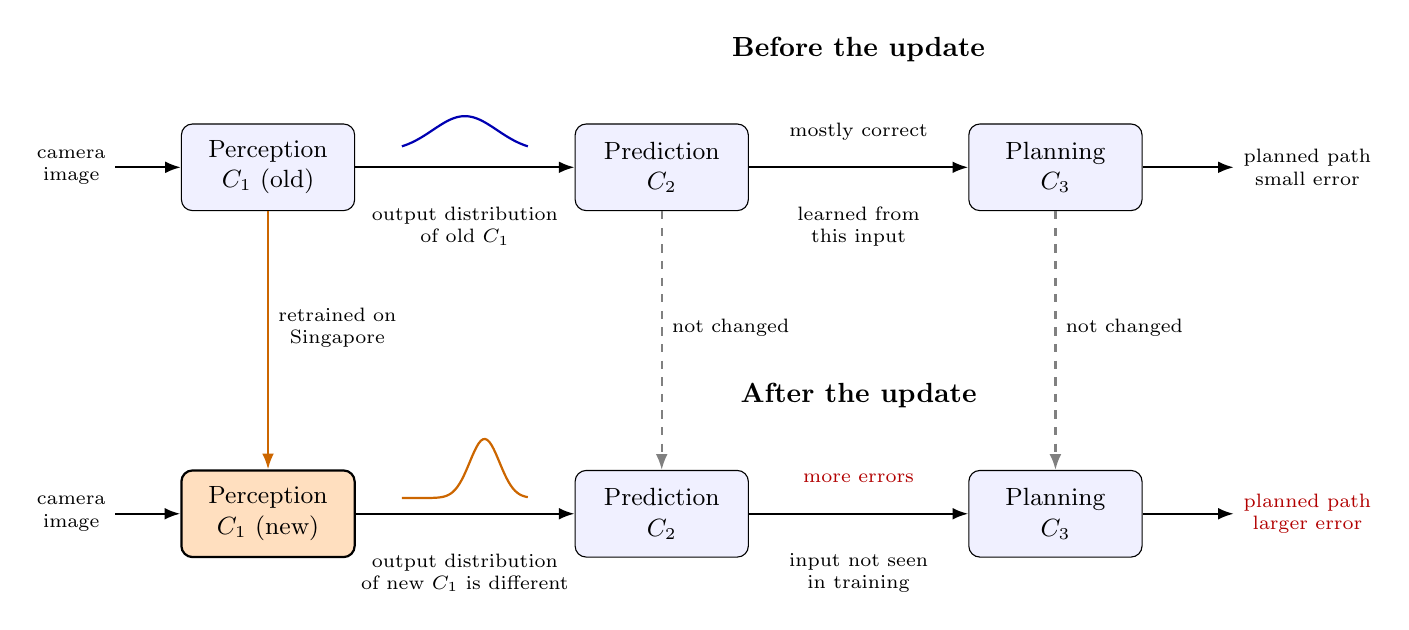
\begin{tikzpicture}[
    font=\small,
    mod/.style={draw, rounded corners, minimum width=22mm, minimum height=11mm,
                align=center, fill=blue!6},
    newmod/.style={mod, fill=orange!25, thick},
    arr/.style={-{Latex[length=2mm]}, thick},
    note/.style={font=\scriptsize, align=center},
]
% x positions: C1 = 0, C2 = 5, C3 = 10; gaps are centred at 2.5 and 7.5
% ---------------- top row: before the update ----------------
\node[font=\bfseries] at (7.5,1.5) {Before the update};
\node[note] (in1) at (-2.5,0) {camera\\image};
\node[mod] (a1) at (0,0) {Perception\\$C_1$ (old)};
\node[mod] (b1) at (5,0) {Prediction\\$C_2$};
\node[mod] (c1) at (10,0) {Planning\\$C_3$};
\node[note] (o1) at (13.2,0) {planned path\\small error};
\draw[arr] (in1) -- (a1);
\draw[arr] (a1) -- (b1);
\draw[arr] (b1) -- (c1);
\draw[arr] (c1) -- (o1);
\draw[blue!70!black, thick, domain=-0.8:0.8, samples=40]
    plot ({2.5+\x}, {0.2+0.45*exp(-3*\x*\x)});
\node[note] at (2.5,-0.75) {output distribution\\of old $C_1$};
\node[note] at (7.5,0.45) {mostly correct};
\node[note] at (7.5,-0.75) {learned from\\this input};

% ---------------- bottom row: after the update ----------------
\node[font=\bfseries] at (7.5,-2.9) {After the update};
\node[note] (in2) at (-2.5,-4.4) {camera\\image};
\node[newmod] (a2) at (0,-4.4) {Perception\\$C_1$ (new)};
\node[mod] (b2) at (5,-4.4) {Prediction\\$C_2$};
\node[mod] (c2) at (10,-4.4) {Planning\\$C_3$};
\node[note, text=red!70!black] (o2) at (13.2,-4.4) {planned path\\larger error};
\draw[arr] (in2) -- (a2);
\draw[arr] (a2) -- (b2);
\draw[arr] (b2) -- (c2);
\draw[arr] (c2) -- (o2);
\draw[orange!80!black, thick, domain=-0.8:0.8, samples=60]
    plot ({2.5+\x}, {-4.2+0.75*exp(-14*(\x-0.25)*(\x-0.25))});
\node[note] at (2.5,-5.15) {output distribution\\of new $C_1$ is different};
\node[note, text=red!70!black] at (7.5,-3.95) {more errors};
\node[note] at (7.5,-5.15) {input not seen\\in training};

% ---------------- links between the rows ----------------
\draw[arr, orange!80!black] (a1.south) -- node[note, right, text=black, pos=0.45] {retrained on\\Singapore} (a2.north);
\draw[arr, dashed, gray] (b1.south) -- node[note, right, text=black, pos=0.45] {not changed} (b2.north);
\draw[arr, dashed, gray] (c1.south) -- node[note, right, text=black, pos=0.45] {not changed} (c2.north);
\end{tikzpicture}}
\caption{One update that shows entangled enhancement}
\label{fig:h1}
\end{figure}

Figure~\ref{fig:h1} shows one update of this kind. Only the perception
module $C_1$ is retrained. The new $C_1$ finds objects more accurately, but
the distribution of the output of $C_1$ changes, shown by the different
curve. The prediction module $C_2$ and the planning module $C_3$ are not
changed and were trained on the output of the old $C_1$. After the update,
$C_2$ and $C_3$ receive an input that differs from the input seen during
training. $C_2$ and $C_3$ then make more errors, and the planning error
increases.

\paragraph{H2 (symptom):} H2 states that the change in the output distribution of $C_1$ and
of $C_2$ after an update is a symptom of entangled enhancement. The change is measured on the
same test images before and after the update. The change is larger in the
updates that meet condition~\eqref{eq:h1} than in the updates that do not.
The improvement $\delta_1$ of $C_1$ alone does not separate the two groups
of updates.

If H2 holds, the engineer who maintains the MLS can compute the change in
the output distribution of $C_1$ and $C_2$ on unlabelled images before
using an update. A large change then warns the engineer that the
downstream modules need retraining as well. The different curve in
Figure~\ref{fig:h1} is the quantity that H2 measures. The set of updates
used to test H1 and H2 also gives the fraction of updates that meet
condition~\eqref{eq:h1}. This fraction is a measured value of $1 - c_1$.

% ============================================================================
\section{Experimental Design}
\label{sec:design}
% ============================================================================

This section describes how the experiment tests H1 and H2. The reduced
dataset keeps the experiment within the available computers. The four
pipelines test whether the effect depends on the choice of models. The
three ways of training $C_2$ and $C_3$ separate the two causes of harm.
The measures of output change test H2, and the checks keep the
measurement valid.

\subsection{Dataset}
\label{sec:data}

The earlier experiments loaded all $850$ scenes of nuScenes, a $45$\,GB
dataset, and used $559$ of these scenes. This size made each experiment too
slow and too large for the available computers. We built a reduced dataset
of $350$ scenes that keeps only the full-size images of the front camera and
the label files, with a size of $4.6$\,GB. Table~\ref{tab:data} compares the
two datasets. The $50$ test scenes are the same as in the earlier
experiments, and the new results can therefore be compared with the old
results.

Boston is split into two separate groups of scenes, one to train $C_1$ and
one to train $C_2$ and $C_3$. A perception module is much more accurate on
the scenes used to train that perception module~\cite{xu2024realworld}.
$C_2$ and $C_3$ must learn from the realistic mistakes of $C_1$, and the
two groups of scenes must therefore be separate. A first run will retrain
the old $C_1$ with two random seeds to show whether $350$ scenes are
enough. If $350$ scenes are not enough, we will add scenes.

\begin{table}[h!]
\centering
\caption{The dataset of the earlier experiments and the reduced dataset.
Every scene gives about $40$ front-camera images. No image is missing in
the reduced dataset.}
\label{tab:data}
\small
\renewcommand{\arraystretch}{1.3}
\begin{tabular}{@{}L{4.6cm}cc@{}}
\toprule
\textbf{Used for} & \textbf{Earlier experiments} & \textbf{Reduced dataset} \\
\midrule
Training the old $C_1$ (Boston) & $280$ scenes & $100$ scenes, $4{,}008$ images \\
Training $C_2$ and $C_3$ (Boston) & none, fixed rules & $100$ scenes, $4{,}046$ images \\
Updating $C_1$ (Singapore) & $229$ scenes & $100$ scenes, $3{,}997$ images \\
Testing (Singapore) & $50$ scenes & the same $50$ scenes, $2{,}020$ images \\
\midrule
\textbf{Scenes used} & $\mathbf{559}$ & $\mathbf{350}$ \\
\textbf{Size of the dataset} & $\mathbf{45}$\,\textbf{GB} & $\mathbf{4.6}$\,\textbf{GB} \\
\bottomrule
\end{tabular}
\end{table}

\subsection{ML Models and Pipelines}
\label{sec:models}

H1 claims that entangled enhancement occurs in several pipelines, not only
in one choice of models. We therefore select two published ML models for
each downstream module and combine the models into four pipelines, shown
in Table~\ref{tab:models}. All four models have public code. $C_1$ is
YOLOv11n in every pipeline. Pipeline P1 is run first, and the other three
pipelines are run once P1 has produced a result.

For $C_2$, the first model is AutoBot-Ego~\cite{girgis2022autobots}, a small
neural network with about $1.5$ million learned numbers. AutoBot-Ego was
trained on all of nuScenes in about $3$ hours on one graphics card.
AutoBot-Ego takes the positions of the objects found in the last few images
and predicts where each object will move. AutoBot-Ego can also learn which
found objects are the same object in different images~\cite{weng2022whose}.
The second model is Social-LSTM~\cite{alahi2016social}, an older and simpler
network that reads the past positions of each object one step at a time.
Social-LSTM needs the same object to be matched across images first. A
second small neural network, which we call the matching network, learns
the matching from the object
identities labelled in nuScenes.

For $C_3$, the first model is PlanT~\cite{renz2022plant}, a small neural
network that takes a list of objects and outputs the planned path. Here
the list holds the positions predicted by $C_2$. The second model is
AD-MLP~\cite{zhai2023rethinking}, the simplest published planning model for
nuScenes. We add the predicted positions of the nearest objects to the
input of AD-MLP. Neither planning model receives the speed of the ego
vehicle as input, because a planning module with this input can ignore the
objects~\cite{zhai2023rethinking,li2024egostatus}.

Before any update is run, we remove the objects from the input of each
trained planning model and check that the planned path changes. A planning
model that ignores the objects cannot be affected by $C_1$, and H1 cannot
be tested with such a model. A model is replaced only if the model fails
to train or ignores the objects.

\begin{table}[h!]
\centering
\caption{The four pipelines built from two ML models for each downstream
module. $C_1$ is YOLOv11n in every pipeline.}
\label{tab:models}
\small
\renewcommand{\arraystretch}{1.3}
\begin{tabular}{@{}lL{5.2cm}L{5.2cm}@{}}
\toprule
\textbf{Pipeline} & \textbf{Prediction module $C_2$} & \textbf{Planning module $C_3$} \\
\midrule
P1 & AutoBot-Ego~\cite{girgis2022autobots} & PlanT~\cite{renz2022plant} \\
P2 & AutoBot-Ego~\cite{girgis2022autobots} & AD-MLP~\cite{zhai2023rethinking}, with object positions added \\
P3 & Social-LSTM~\cite{alahi2016social}, with the matching network & PlanT~\cite{renz2022plant} \\
P4 & Social-LSTM~\cite{alahi2016social}, with the matching network & AD-MLP~\cite{zhai2023rethinking}, with object positions added \\
\bottomrule
\end{tabular}
\end{table}

\subsection{Three Ways of Training $C_2$ and $C_3$}
\label{sec:settings}

The two causes of Section~\ref{sec:background} predict different results
when $C_2$ and $C_3$ learn from different inputs. When the ego vehicle
drives, the modules are always connected in the pipeline. The output of
$C_1$ goes to $C_2$, and the output of $C_2$ goes to $C_3$. Training happens
earlier, and each module is trained separately. During training we choose
the input of each module. The input of $C_2$ can be the ground truth, or
the output of $C_1$, including the mistakes of $C_1$. We therefore train
$C_2$ and $C_3$ in the three ways shown in Table~\ref{tab:settings}. After
training, the modules are connected into the normal pipeline in all three
cases, and the same update of $C_1$ is applied.

\begin{table}[h!]
\centering
\caption{The three ways of training $C_2$ and $C_3$. Only the input seen
during training differs. When the ego vehicle drives, the modules are
connected in the same pipeline in all three cases.}
\label{tab:settings}
\small
\renewcommand{\arraystretch}{1.3}
\begin{tabular}{@{}L{4.6cm}L{8.6cm}@{}}
\toprule
\textbf{$C_2$ and $C_3$ learn from} & \textbf{Expected result if the first cause acts} \\
\midrule
the ground truth & a better $C_1$ decreases the planning error or changes nothing \\
the output of the old $C_1$ & the planning error increases, and increases more than after training on the ground truth \\
the output of the new $C_1$ & the increase seen after training on the old $C_1$ disappears \\
\bottomrule
\end{tabular}
\end{table}

When $C_2$ and $C_3$ learn from the ground truth, $C_2$ and $C_3$ have never
seen the mistakes of any $C_1$. When $C_1$ improves, the output of $C_1$
comes closer to the ground truth, and the planning error should decrease
or stay the same. When $C_2$ and $C_3$ learn from the output of the old
$C_1$, $C_2$ and $C_3$ also adapt to the mistakes of the old $C_1$. The
first cause can act only in this case, and the planning error should
increase more than after training on the ground truth.

When $C_2$ and $C_3$ are trained again on the output of the new $C_1$, the
old mistakes are no longer part of the training data. If the first cause
produced the increase, the increase should disappear. If the planning
error still increases, the second cause acts, and splitting $\delta_1$ by
object type and by distance will show where $C_1$ became worse. Both causes
can act at the same time. H1 is rejected if the planning error and the
prediction error increase beyond random variation in no update, in no
training case and in no pipeline.

\subsection{Measures of Output Change}
\label{sec:symptom}

H2 needs a number that describes how much the output of a component
changes after an update, without the ground truth. For each update we
compare the output of the old component with the output of the new
component on the same $2{,}020$ test images. Table~\ref{tab:measures}
lists the measures. For $C_1$ we compare the
number of objects found per image and the mix of object types with the
Jensen--Shannon divergence. We compare the confidence scores and the sizes
and positions of the found objects with the Wasserstein distance. We also
count the fraction of objects that only one of the two versions of $C_1$
finds on the same image.

For $C_2$ we compute the Wasserstein distance between the predicted
movements before and after the update. We also compute the average
distance between the positions predicted before and after the update for
the same object. The rank correlation between each measure and $\Delta_3$
is a number between $-1$ and $1$. The rank correlation is close to $1$
when a higher measure always comes with a larger $\Delta_3$. H2 is
supported if the measures are clearly higher in the updates that meet
condition~\eqref{eq:h1}, and if the measures separate the two groups of
updates better than $\delta_1$ does. H2 is rejected if no measure
separates the two groups better than $\delta_1$.

\begin{table}[h!]
\centering
\caption{Measures of output change used to test H2. Every measure compares
the old and the new version on the same test images and needs no ground
truth.}
\label{tab:measures}
\small
\renewcommand{\arraystretch}{1.3}
\begin{tabular}{@{}lL{6.4cm}L{5.4cm}@{}}
\toprule
\textbf{Output} & \textbf{What is compared} & \textbf{Measure} \\
\midrule
$C_1$ & number of objects found per image & Jensen--Shannon divergence \\
$C_1$ & mix of object types & Jensen--Shannon divergence \\
$C_1$ & confidence scores of the found objects & Wasserstein distance \\
$C_1$ & sizes and positions of the found objects & Wasserstein distance \\
$C_1$ & objects found by only one of the two versions & fraction of such objects \\
\midrule
$C_2$ & predicted movements & Wasserstein distance \\
$C_2$ & predicted positions of the same object & average distance between the old and the new prediction \\
\bottomrule
\end{tabular}
\end{table}

\subsection{Checks on the Measurement}
\label{sec:checks}

\paragraph{Unchanged modules:} We measure each downstream module in two
ways. In the first way the module receives the ground truth as input. In
the second way the module receives the output of the preceding module.
The update does not change $C_2$ and $C_3$. The result of $C_2$ and $C_3$
with the ground truth as input must therefore stay exactly the same, digit
by digit. A change in this result shows a fault in the measurement.

\paragraph{Random variation and planning measures:} An increase of the
planning error counts only if the increase is larger than the increase
produced by random variation. The same rule decides whether the smallest
increase in the earlier experiments, $0.008$\,m, is real. We also report
the planning error together with the collision rate, which is the fraction
of scenes in which the planned path hits an object. The earlier
experiments showed that the planning error and the collision rate can move
in opposite directions after the same update.

% ============================================================================
\section{Conclusion}
% ============================================================================

The earlier experiments in this study showed that retraining the
perception module can increase the planning error. The downstream modules
in those experiments were fixed rules and could not show the cause that
the theory of entangled enhancement describes. This report states H1, that
an update of the perception module can reduce the performance of the ML
prediction module and the ML planning module in several pipelines. The
report also states H2, that the change in the output distribution of the
perception module and the prediction module, measured without ground
truth, is a symptom of entangled enhancement.

A symptom that needs no ground truth can be computed before an update is
used, and H2 is therefore the hypothesis closest to a maintenance method.
The three ways of training separate the two causes, the four pipelines
test whether the effect depends on the choice of models, and the checks
keep the measurement valid. The reduced dataset is built. The next step is
the first run with two random seeds of the old $C_1$ on the reduced
dataset.

\FloatBarrier
\bibliographystyle{IEEEtran}
\bibliography{references}

\end{document}
